%% intro.tex
Machine learning (ML) has become an indispensable part of our everyday lives.
For example, we use it for machine translation, transport and logistics organization, product recommendations, fraud detection, self-driving cars, and much more.
Machine Learning uses mathematical functions to map an input to an output.
These functions usually extract patterns from the input data to build a relationship between input and output.
The term Machine Learning stems from the fact that we use \emph{machines} to correlate the input and the output to a function (i.e. to \emph{learn} a function) during a training period.
A sub-branch of Machine Learning is Deep Learning (DL).
DL algorithms are able to learn hidden patterns within data to make predictions.
They benefit from the accelerated computing power and big data made available in the last decade.
Deep Learning is considered state-of-the-art for many learning tasks especially for high-dimensional data.
Typical high-dimensional data are texts, audio recordings, 2D as well as 3D images, and videos.
Deep Learning models use artificial neural networks to learn the mapping function between given input and output data.
In the following, the fundamentals of Deep Learning is explained.
Only those aspects that are relevant for the understanding of the rest of the thesis are discussed.


\section{Fundamentals}\seclbl{fundamentalsDL}
The idea for artificial neural networks (ANN) stems from biology and aims to capture the interaction of brain cells (neurons) with a mathematical model.
A first model for a neuron was proposed by MuCulloch and Pitts in 1943 \sidecite{McCulloch_Pitts_1943}.
Similar to how a"neuron of the human brain transmits electrical impulses through the nervous system, the artificial neuron of MuCulloch and Pitts receives multiple input signals and transforms them into a output signal.
A neuron takes an input vector \(\boldsymbol{x} = (x_1, ..., x_n)\) where \(x_i \in \{0, 1\}\) and maps it to an output \(\hat{y} \in \{0, 1\}\).
The mapping from the input to the output is done by using an aggregation function \(g\) that sums up the input vector \(\boldsymbol{x}\) and a activation function \(f\) that outputs \(1\) if the output of \(g\) is greater than a threshold \(\theta\) and \(0\) otherwise.

\begin{equation}\eqlbl{McCulloch_Pitts_agg}
	g(\boldsymbol{x}) = g(x_1, ..., x_n) = \sum_{i=1}^{n}x_i\\
\end{equation}
\begin{equation}\eqlbl{McCulloch_Pitts_act}
		\hat{y} = f(g(\boldsymbol{x})) = \begin{cases}
      		1, & \text{if}\ g(x) \geq \theta \\
      		0, & \text{otherwise}
    	\end{cases}
\end{equation}%

In 1958, Rosenblatt \sideciteay{Rosenblatt_1958} developed the Perceptron which works with real numbers as input.
The input vector \(\boldsymbol{x} = (x_1, ..., x_n)\) where \(x_i \in \mathbb{R}^n\) is multiplied with a weight vector \(\boldsymbol{w} = (w_1, ..., w_n)\) where \(w_i \in \mathbb{R}^n\) with the same length.

\begin{equation}\eqlbl{Perceptron_agg}
	g(\boldsymbol{x}) = g(x_1, ..., x_n) = \sum_{i=1}^{n} w_i \cdot x_i\\
\end{equation}

The output \(\hat{y} \in \{0, 1\}\) is similar to the MuCulloch and Pitts neuron \(1\) if the aggregated value is greater than a threshold \(\theta\) and \(0\) otherwise as described in equation \ref{McCulloch_Pitts_act}. The equations \eqref*{Perceptron_agg} and \eqref*{McCulloch_Pitts_act} can be rewritten as


\begin{equation}\eqlbl{Perceptron}
		\hat{y} =f(g(\boldsymbol{x})) = \begin{cases}
      		1, & \text{if}\ \sum_{i=1}^{n}w_i \cdot x_i - \theta \geq 0 \\
      		0, & \text{otherwise}
    	\end{cases}
\end{equation}

Later, the step-function \(f\) was replaced with other functions so that the output could also be a real number \(\hat{y} \in \mathbb{R}\). Often used functions are

\begin{equation}\eqlbl{act_functions}
	\begin{aligned}
		\text{Sigmoid: } \sigma(z) = \frac{1}{1+\mathrm{e}^{-z}}\\
		\text{Rectified linear unit (ReLU): } (z)^{+} = \max{0, z}\\
		\text{Hyperbolic tangent (tanh): } \tanh(z) = \frac{\mathrm{e}^{z}-\mathrm{e}^{-z}}{\mathrm{e}^{z}+\mathrm{e}^{-z}}
	\end{aligned}
\end{equation}

By convention, instead of using the threshold \(- \theta\) often a bias \(b\) is used which leads to:

\begin{equation}\eqlbl{nn}
	\begin{aligned}
		z = g(\boldsymbol{x}) = \boldsymbol{w} \cdot \boldsymbol{x} = \sum_{i=1}^{n}w_i \cdot x_i + b\\
		\hat{y} = f(z)
	\end{aligned}
\end{equation}

However, the brain consists of multiple neurons which are connected through synapses.
Therefore, ANNs consist not only of one neuron but combine multiple neurons in a network. 
These neurons are organized into layers.
A shallow neural network consists of one hidden layer in which the input \(\boldsymbol{x}\) is fed to calculate the output \(\boldsymbol{\hat{y}}\)%\sidenote{\(\boldsymbol{\hat{y}}\) has become a vector since multiple neurons produce multiple output values}.
The universal approximation theorem of Cybenko \sidecite{Cybenko_1989} proves that a shallow network with enough neurons can approximate any mapping function between inputs and outputs.
However, very complex mapping functions may need too many hidden neurons.
The neurons of the hidden layer extract features in the input space.
Since only one layer is used, the features cannot be hierarchically organized and become complex enough.

A multi-layer perceptron (MLP), on the other hand, consists of multiple layers.
The different layers extract increasingly complex features.
In a MLP. the input \(\boldsymbol{x}\) is fed into the first layer, each subsequent layer \(l\) gets the output of the previous layer \(l-1\) as input.
In the following, we describe the mathematical model for fully connected layers, where all neurons of a layer are connected with the subsequent layer%\sidenote{many modern network architectures are not fully connected and can have either missing or recurrent connections}.
For a MLP with \(m\) layers, we define the output of the aggregation \(g\) as \(\boldsymbol{z}^{[l]}\) and the output the activation function as \(\boldsymbol{a}^{[l]}\) for layer \(l\).
Furthermore, we use \(\boldsymbol{w}^{[l]}\) for the weight vector and \(b^{[l]}\) for the bias of layer \(l\).
Thus, the mathematical model of a MLP is defined as

\begin{equation}\eqlbl{mlp}
	\begin{aligned}
		\boldsymbol{z}^{[l]} = \boldsymbol{w}^{[l]}\boldsymbol{a}^{[l-1]} + b^{[l]}\\
		\boldsymbol{a}^{[l]} = f({z}^{[l]})
	\end{aligned}
\end{equation}

Since the input is fed into the first layer and the output is the result from the last layer \(\boldsymbol{x} = {a}^{[0]}\) and \(\boldsymbol{\hat{y}} = {a}^{[m]}\) holds true.

So far, only the forward-pass which is used to calculate the output \(\boldsymbol{\hat{y}}\) was discussed.
However, the model output \(\boldsymbol{\hat{y}}\) will only be close to the target output \(\boldsymbol{y}\) if the weights \(\boldsymbol{w}^{[l]}\) and biases \(b^{[l]}\) are properly defined.
These parameters are learned during a training period.
The training can take place in a supervised, semi-supervised, self-supervised, unsupervised, or reinforcement learning based manner.
In supervised learning, the output of the model \(\boldsymbol{\hat{y}}\) for a given input \(\boldsymbol{x}\) is compared to manually created target outputs \(\boldsymbol{y}\).
Unsupervised learning, on the other hand, tries to find patterns in the input \(\boldsymbol{x}\) and to cluster the samples into meaningful groups without using target labels.
Semi-supervised learning is a hybrid approach of the the aforementioned principles that combines a small amount of labelled data with a large amount of unlabelled data.
In self-supervised learning, the target outputs \(\boldsymbol{y}\) are directly derived from the input data \(\boldsymbol{x}\) (e.g. predict a masked part of the input \(\boldsymbol{x}\)).
Lastly, reinforcement learning algorithms aim to maximize a reward that they become from an environment based on some action they executed.

These learning principle have in common that a loss function \(\mathcal{L}\) can calculate a loss value based on the model output \(\boldsymbol{\hat{y}}\). 
For example, the mean square error (MSE) can be used for regression problems or the negative log-likelihood for classification problems.
The chosen loss function is minimized interatively with stochastic gradient descent (SGD)%\sidenote{There exist also other optimizer methods such as SGD with momentum, RMSprop, or Adam \citep{Kingma2015AdamAM}} until the network converges.
The idea behind stochastic gradient descent is to make use of the fact that the negative gradient of the loss value points to the direction of the steepest descent (i.e. in the direction where the loss gets smaller).
SGD therefore updates the network parameters by taking a step of size \(\eta\) in the direction of their negative gradient

\begin{equation}\eqlbl{sgd}
	\begin{aligned}
		\Delta \boldsymbol{w}^{[l]} = -\eta \nabla_{\boldsymbol{w}^{[l]}} \mathcal{L}\\
		\Delta b^{[l]} = -\eta \nabla_{b^{[l]}} \mathcal{L}
	\end{aligned}
\end{equation}

The gradients of the weights \(\boldsymbol{w}^{[l]}\) and biases \(b^{[l]}\) can efficiently be calculated with an algorithm called backpropagation \sidecite{Rumelhart_Hinton_Williams_1986}, which is just a smart implementation of the chain rule%\sidenote{While a detailed discussion on backpropagation is out of scope for this thesis, we refer interested reader to the Deep Learning course by Andrew Ng \cite{Coursera}}.

TODO: Describe CNN, Transformer, ... etc.???

\section{Limitations of Deep Learning}\seclbl{limitationsDL}
The rise of Deep Learning over the past decade has only been possible because of major technological advances in hardware.
Moore’s law \cite{Moore_2006} states that the number of transistors in a dense integrated circuit doubles about every two years and is the only known physical process following an exponential curve.
An analysis by OpenAI shows that since 2012 the amount of compute has even increasing exponentially with a doubling time  of \(3.4\) months \cite{OpenAI_compute}.
However, the exponential increase seems to come to an end since the size of transistors hit physical limitations.
It is assumed that Moore's law will end by around 2025 \sidecite{Kumar_2015}.
Besides the progress in the field, Deep Learning methods also became better because they grew exponentially.
They not only have more layers and more parameters but also require more data.
Even the growth in the last five years is astonishing.
While the state-of-the-art language model from 2018 \sidecite{Peters_Neumann_Iyyer_Gardner_Clark_Lee_Zettlemoyer_2018} had around \(94\)M parameters, the state-of-the-art in 2020 \sidecite{NEURIPS2020_1457c0d6} already had \(175\)B parameters. Training such a model on a single V100 GPU would take about 355 years and cost about \(4.6\)M dollars \cite{Lambda_GPT3}.
A recent language model from Microsoft and Nvidia \sidecite{Shoeybi_Patwary_Puri_LeGresley_Casper_Catanzaro_2020} even has \(530\)B parameters.
Only a few institutions with massive resources are able to train such big models.
In general, inference on low-budget hardware such as smartphones or embedded hardware becomes prohibitive with the growing size of deep networks.
Even tough there exist techniques to shrink the model size after training such as quantization \cite{Wu_Judd_Zhang_Isaev_Micikevicius_2020}, model pruning \cite{Choudhary_Mishra_Goswami_Sarangapani_2020}, or model distillation \cite{Hinton_Vinyals_Dean_2015} it is questionable if making models bigger is the best way to develop intelligent systems.

Another major issue of Deep Learning systems is that they suffer from catastrophic forgetting.
If a model is trained on a specific task and afterwards trained (or fine-tuned) on another task, the model suffers a ``catastrophic'' drop in performance over the first task.
The reason for this effect is that the model during training on the second task adjusts the parameters learned during the first task and therefore ``forgets'' the learned mapping functions.
Just mixing all datasets or to learn all tasks in parallel in a current multi-task setup \cite{Zhang_Yang_2021} doesn't seem feasible to achieve some kind of general intelligence as this involves too many different unrelated tasks.
Catastrophic forgetting is also caused by the fact that learning is mostly done offline%\sidenote{Offline in this context means that the model parameters are not adapted after training during inference time}.
Online learning \cite{Sahoo_Pham_Lu_Hoi_2017} and lifelong learning \cite{Parisi_Kemker_Part_Kanan_Wermter_2019} are currently hot research topics.
However, these methods have not yet been established.

Furthermore, there exists problems which may cannot be solved with the current principles used for Deep Learning.
First of all, it is questionable if Deep Learning models can achieve \emph{real} generalization%\sidenote{Generalization refers to the ability of the model to adapt properly to previously unseen data from the same distribution}.
With enough data, can achieve generalization in the sense that the model can interpolate within the data distribution.
However, deep learning models fail to extrapolate.
For example, convolutional neural networks (CNNs) do not generalize to different viewpoints unless they are added to the training data \sidecite{Madan_Henry_Dozier_Ho_Bhandari_Sasaki_Durand_Pfister_Boix_2022}.

Second, Deep Learning is not able to learn abstract relationships in a few trials but requires many samples of it and is thus data hungry.\sidenote{Delme!!!}
Marcus Gary \sidecite{Marcus_2018} argues that if he tells that a ``schmister'' is a sister over the age of 10 but under the age of 21, humans can  immediately infer whether they or their best friends have any ``schmister''. However, modern DL systems lacks a mechanism for learning abstractions through explicit, verbal definition and require thousands or even more training samples.

Third, no DL model has been able to demonstrate causal reasoning in a generic way.
Deep Learning models find correlations between the inputs and the outputs, but not the causation.
Other AI approaches such as hierarchical Bayesian computing or probabilistic graphical models are better at causal reasoning but cannot be well combined with Deep Learning models.

Lastly, Deep Learning models are to some extend too isolated since they have no embodiment and cannot interact with the world.
For example, the human body provides needs, goals, emotions, and gut feeling%\sidenote{one could argue that the body is therefore even a co-processor of the brain}.
In current Deep Learning systems are emotions totally absent and the goals are set externally.
Deep Reinforcement Learning can be considered as a first step in the direction of dissolving this isolation, as they interact with a virtual environment. 
AI systems that interact with the real world do not work well so far.
Moravec's paradox \sidecite{Moravec_1995} states that ``it is comparatively easy to make computers exhibit adult level performance on intelligence tests or playing checkers, and difficult or impossible to give them the skills of a one-year-old when it comes to perception and mobility''.


\section{Biological Learning}\seclbl{biological_learning}
The human brain comprises many interconnected areas processing everything in parallel.
For example, Figure \figref{visual_cortext} illustrates the connections between different organizational units in the cerebral cortex which are responsible for vision.
It can be seen that these areas are connected in a rather complex structure.
\begin{figure}[h]
    \centering
    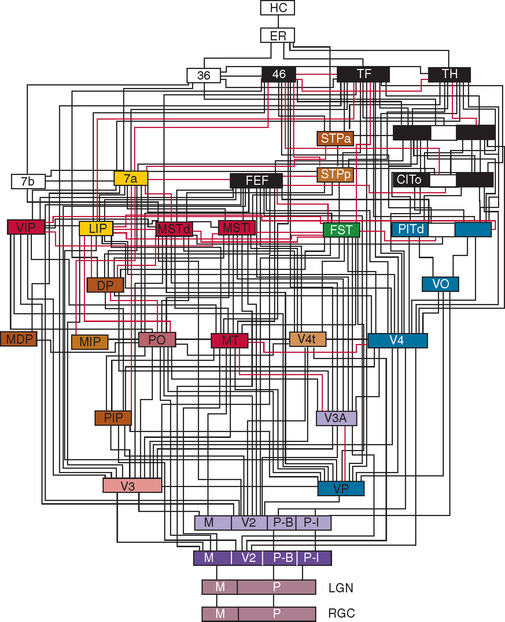
\includegraphics[width=0.99\textwidth]{felleman_visual_cortex}
    \caption[Organization of the visual system in the cerebral cortex]{The organization of the visual system in the cerebral cortex. The image is from \citeay{Felleman_Van_Essen_1991}.}
    \figlbl{visual_cortext}
\end{figure}
Deep Learning architectures, on the other hand, are mostly unidirectional and the signal flows unidirectional from layer to layer%\sidenote{Except for recurrent connections, skip-connections, or residual-connections}.
However, the choice of the architecture influences the how the model can learn the mapping function from input to output.
It could be that the complex structure of our brain comprises an inductive bias which was learned over time through evolution.

A learning system requires a mechanism that tells the system if something goes well or wrong so that it can learn from it.
This is called the \emph{credit assignment problem}.
Backpropagation (c.f. Section \secref*{fundamentalsDL}) solves this problem by propagating the error backwards through the network.
However, information flows in the brain only in one direction from the presynaptic neurons to the postsynaptic neurons.
Therefore, backpropagation is not biologically plausible.
Lillicrap et al. \sidecite{Lillicrap_Cownden_Tweed_Akerman_2016} shows that an additional set of random feedback weights is able to transmit useful gradients.
Their work has reopend questions how the brain could process error signals and has dispel some long-held assumptions about algorithmic constraints on learning.

Not only the structure of the network and the way how the feedback is calculated is different between biological learning and Deep Learning.
Also the neurons themselves are different.
While the artificial neuron doesn't have any dynamics (c.f. Equation \eqref*{nn}), biological neurons are highly dynamic:
Biological neurons adapt their firing rate to constant inputs, they may continue firing after an input disappears, and can even fire when no input is active.

TODO: Add reference to reservoir computing

Lastly, the neurons in the brain are self-organizing.
This means that a group of elementary units such as neurons or a group of neurons perform similar rule of behavior on a sub-set of the available information.
Such a system doesn't have a central supervision that orchestrates these units.
Each unit applies similar deterministic functions to the information received.
Two important principles of such systems are (i) localized learning which means that each unit adapt their behavior to the information they receive; and (ii) emergence which means that there is no explicit loss function that tells the system what to do.


% \section{Neurocomputing}\seclbl{neurocomputing}


% \section{Motivation}\seclbl{motivation}


% Related work: Hedge Backpropagation: https://arxiv.org/abs/1711.03705



